\begin{figure}[!htbp]
\begin{center}
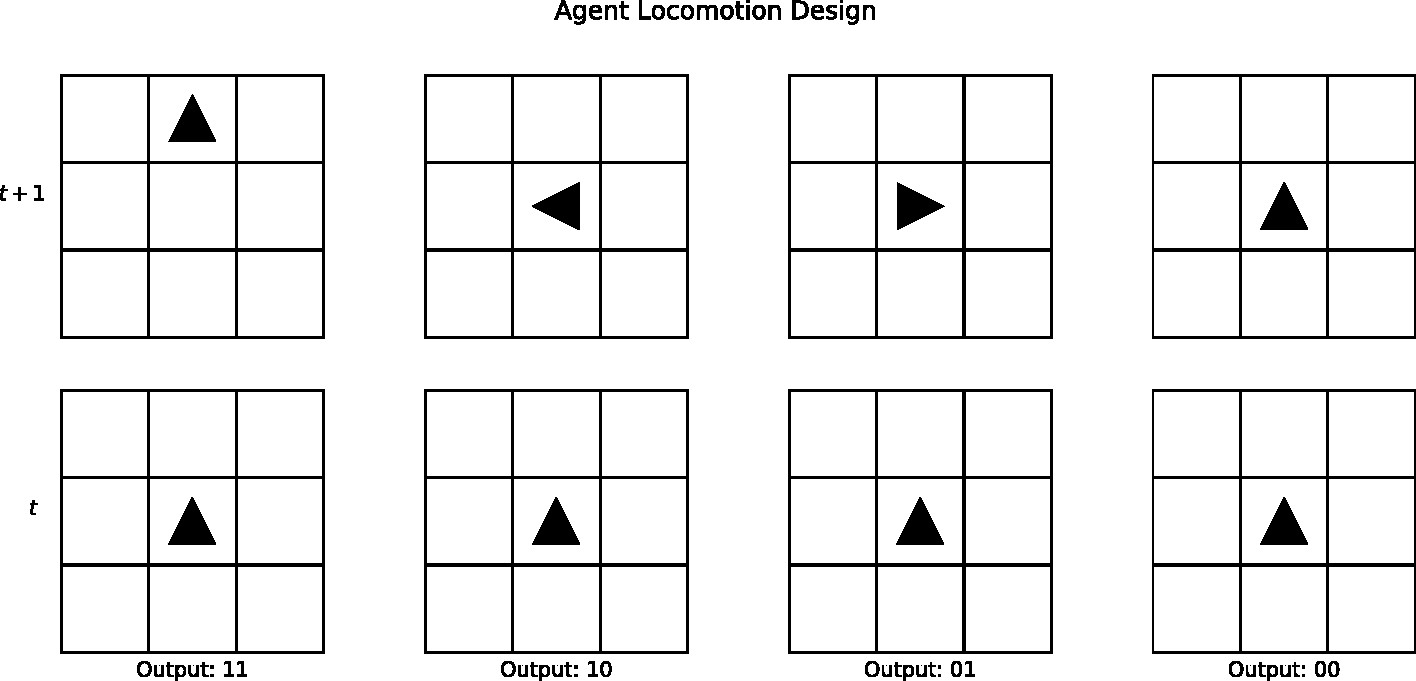
\includegraphics[width=\textwidth]{img/movement_explanatory}
\caption{
Agent locomotion: Image is to be read from bottom to top, with time t at the bottom and time t+1 at the top. \textbf{Outer Left:} Agent moves forward one cell via setting its locomotion bits to '11'. \textbf{Inner Left:} Agent Turns left via '10'. \textbf{Inner Right:} Agent turns right via '01'. \textbf{Outer Right:} Agent may remain stationary by outputing '00'.
}
\label{fig:movement_explanatory}
\end{center}
\end{figure}
